\tightsection{Challenges of Practical Prediction Algorithms}
\label{sec:challenges}

While in previous section we showed that video metrics are predictable with the attributes we collected, there are still several challenges in designing such prediction algorithm in practice. In particular, while predictability tend to increase with more attributes, the data points contained in each fine-grained AC group becomes sparse, and such sparsity is susceptible to noise.

%\xil{the following seems to be only part of the challenge}
%In particular, a practical algorithm can only use the information (quality samples) collected before the minute that the session under prediction belongs to.

First, we categorize the sources of difficulty in predicting video quality accurately (\Section~\ref{subsec:challenges}) which inform the choice of aggregating identical groups of all attributes (i.e., the finest identical groups) by ignoring (hopefully, less important) attributes so that more samples will be used(\Section~\ref{subsec:aggregation}) to counteract the noise and estimation error brought by sparse data.

\tightsubsection{Predicting from finite data}

\label{subsec:challenges}
Although the figures~\ref{fig:predictability} show that in many cases, quality is similar among quality samples that share the same attribute values and same temporal interval, there are still a lot of quality sample groups that have high dispersion. This is one of the key challenges that make quality prediction difficult. 
In this part, we enumerate the potential reasons that causes the dispersion we observe. Intuitively, if the number of similar sessions is small (e.g., $~10$ sessions), the mean quality outcome is subject to considerable random noise.  If we use this mean for prediction, the prediction will be subject to the same noise and consequently to high average error.  As the number of attributes grows, quality grows more predictable (as the noise decreases) but the number of perfectly-matched sessions may drop exponentially.

%Of course, prediction in the presence of limited information is statistics problem, and there are many potential solutions to this problem.  
In general, there are four sources of prediction error:
%Any solution will deal with, and potentially trade off, four sources of prediction error:

\begin{packedenumerate}
  \item \emph{Estimation error:} In the statistical literature, prediction error due to limited data is often called {\it estimation error}.  Even other things being equal, more data produce more accurate prediction. For example, Figure~\ref{fig:group-size-impact} presents the prediction error vs. group size (i.e., number of samples). Given a large number of attributes and the combinatorial nature of the attributes, estimation error is a serious problem in practice. 
  % Using all available attributes, many sessions have very few matches, as we would expect given the exponential explosion in combinations of attribute values.  

\begin{figure}[h!]
\centering
\subfigure[Prediction error vs. group size (w.r.t average bitrate)]
{
        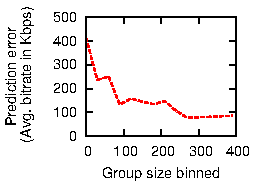
\includegraphics[width=110pt]{figures/count-err.pdf}
	\label{subfig:group-size-impact:count-err}
}
\subfigure[Distribution of group size]
{
        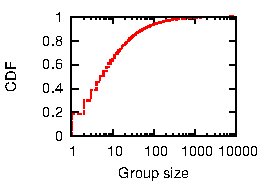
\includegraphics[width=110pt]{figures/count-cdf.pdf}
}
\tightcaption{Impact of group size (i.e., number of samples in a group). They show that more samples give more accuracy, but most of groups do not have sufficient samples for accurate prediction.}
\label{fig:group-size-impact}
\end{figure}

\item \emph{Bias} due to missing or unused information: The bias occurs when we do not observe (or use) an attribute, $X$, that is important for prediction. Then, even if we have infinitely many sessions that match the current session on all observed attributes, the average outcome for all of those sessions may be different from the average outcome for the subset of sessions that match the current session on attribute $X$.  Thus, the bias is not alleviated by gathering more session data, but by gathering more attributes about each session.

\item \emph{Unavailability of recent data:} In a practical system, there are delays in measuring, sending and processing quality samples, so they are not available instantly.  If conditions change rapidly, there may be no quality samples sufficiently close to the session under prediction.  This is an extSreme example of estimation error.  In this case it may be necessary to model the evolution of the video ecosystem over time in order to extrapolate to the current time. Figure~\ref{quality-variability} shows per-minute quality variability. It shows that even with sufficient data, the mean value of a group of quality samples could vary significantly.

\begin{figure}[h!]
\centering
 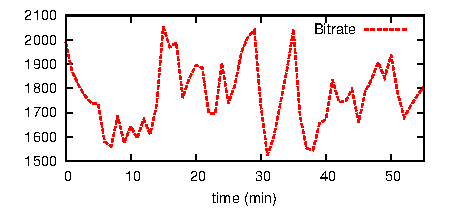
\includegraphics[width=0.4\textwidth] {figures/quality-time.pdf}
\tightcaption{Temporal variability of quality. The figure shows the mean value of average bitrate of a fixed group of same [Site, Initial CDN, Initial Bitrate, ConnectionType, ASN, Object], which has 100 quality samples in every minute in the figure.}
\label{fig:quality-variability}
\end{figure}

  \item \emph{Noise:} Even if we observed all conceivable attributes of a session and had infinitely many examples of exactly quality samples, outcomes may be affected by non-deterministic inputs.  For example, performance may be affected by exponentially backoff at the data link layer or the congestion generated by cross traffic at the network layer. This implies that some degree of prediction error is inevitable.
\end{packedenumerate}

% XIL: I don't see the point of having a formalization, I see no conclusion drawn from it
%Next, we formalize the prediction error (see \cite{domingos2000unified} for a less specialized discussion of the decomposition of prediction error).  Let $D$ be a set of quality samples from which a prediction algorithm learns its predictions.  Let $p_i$ be the predicted quality for session $i$ and $q_i$ be its actual quality.  We further assume that $q_i$ is fixed except for an independent additive noise component, i.e. $q_i = \hat{q}_i + \epsilon_i$, where $\hat{q}_i$ is non-random and $\epsilon_i$ is a random variable with mean $0$, independent of $p_i$.  Then the mean squared prediction error of $p_i$ is:

\comment{
\begin{align}
  \label{eqn:biasvariance}
  \E_D[(p_i - q_i)^2] &= \Var_D[p_i - q_i] + (\E_D[p_i - q_i])^2
\end{align}
\begin{align*}
  \label{eqn:biasvariancelong}
  &= \Var_D[p_i - \hat{q}_i - \epsilon_i] + (\E_D[p_i - \hat{q}_i - \epsilon_i])^2 \\
  &= \Var_D[p_i - \hat{q}_i] + \Var_D[\epsilon_i] + (\E_D[p_i - \hat{q}_i - \epsilon_i])^2\\
  &= \Var_D[p_i] + \Var_D[\epsilon_i] + (\E_D[p_i - \hat{q}_i - \epsilon_i])^2\\
  &= \Var_D[p_i] + \Var_D[\epsilon_i] + (\E_D[p_i - \hat{q}_i] - \E_D[\epsilon_i])^2\\
  &= \Var_D[p_i] + \Var_D[\epsilon_i] + (\E_D[p_i] - \hat{q})^2
\end{align*}
}

%The first term in equation \eqref{eqn:biasvariancelong} is estimation error -- the variability in predictions across possible sets of observed data.  It will increase as the number of sessions similar to session $i$ in $D$ decreases. As a special case, it may be very large if only a few quality samples in $D$ are temporally close to session $i$.  The second term is noise.  The third term is the squared bias of the predictor, which does not generally decrease with the size of $D$.  The average prediction error is simply the average over all these three terms of sessions $i$. 

\tightsubsection{Aggregation}
\label{subsec:aggregation}
A simple strategy to reduce estimation error is {\it aggregation}~\cite{any citation?}.  By aggregation we mean putting quality samples into coarser groups that match on only a subset of observed attributes.  Aggregation increases the number of samples in each identical group by reducing the number of attributes, thus reducing estimation error at the cost of increased bias. 
Intuitively, when estimation error is small (say, when a fine-grained identical group contains many sessions) we want to eliminate bias by using a fine-grained group.  When estimation error is large, we want to aggregate more.  \comment{Figure \fillme demonstrates this for \fillme\jc{nice to have a figure to confirm such tradeoff does happen in our dataset.}.}  This indicates that a prediction algorithm that uses aggregation should pay attention to its error rate to determine the right degree of aggregation.


\begin{figure}[h!]
\centering
 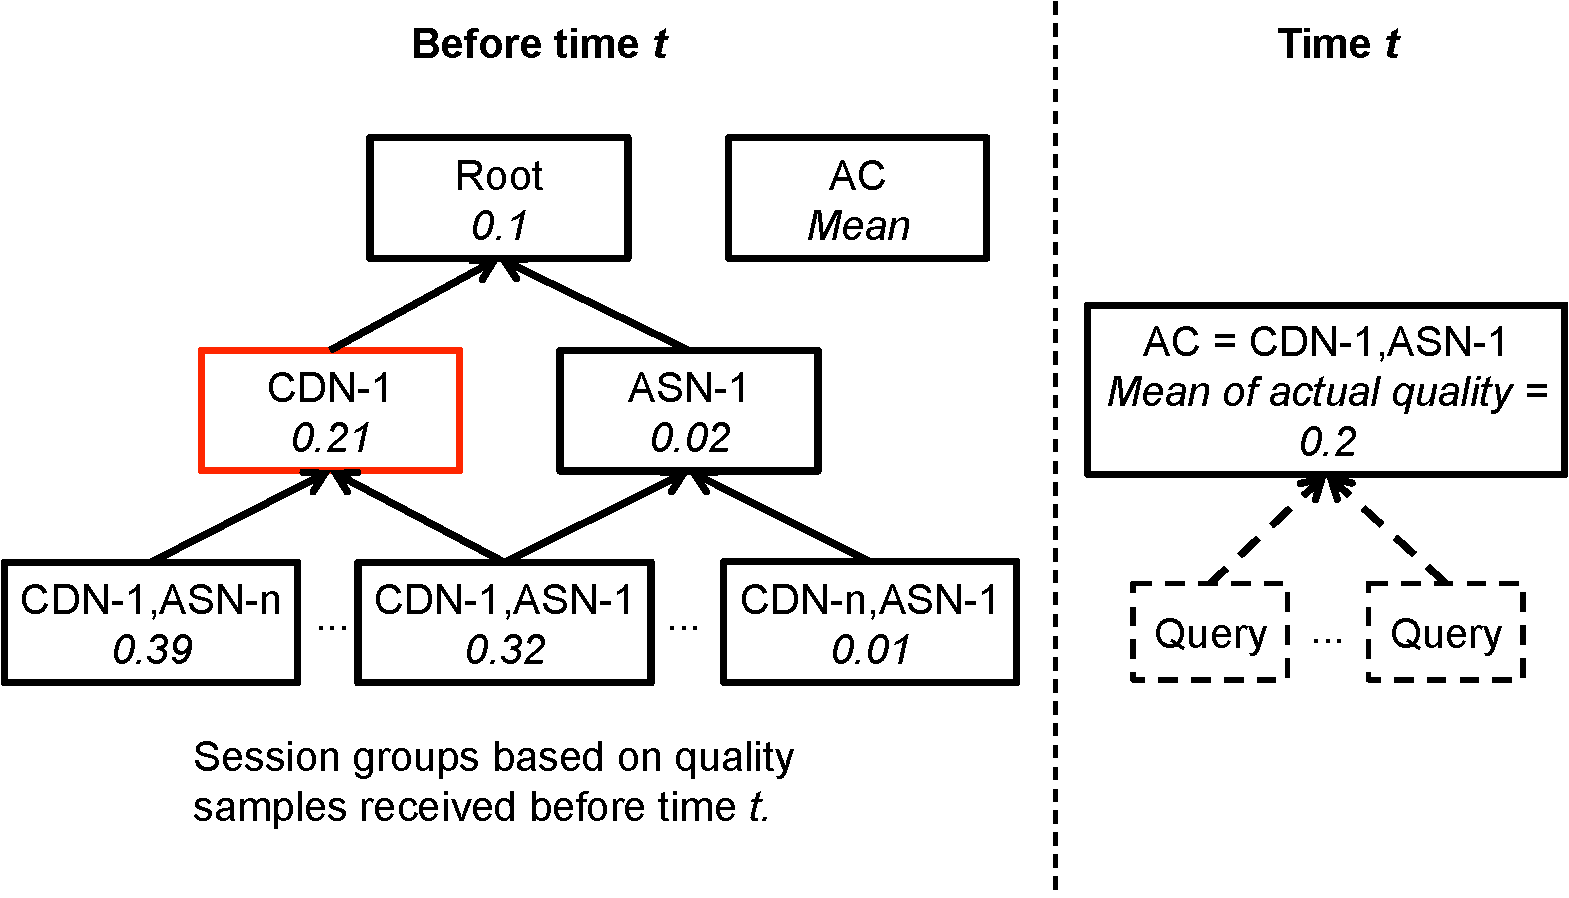
\includegraphics[width=0.5\textwidth] {figures/fig-optimal-AC.pdf}
\tightcaption{Example of how optimal AC is identified. The optimal AC is colored in red. Assuming the considered attributes are fixed, the optimal AC assumes that all sessions that belong to the same finest group should be given the same prediction, and the optimal AC is the one that gives the closest prediction among those that contain this finest group.}
\label{fig:example-optimal-ac}
\end{figure}

We use a simple methodology, called {\it optimal AC}, to show the dynamics of the right degree aggregation. For a finest identical group at $t$-th minute, we first build a hierarchy that consists of all degrees of aggregation over the quality samples we collects before the $t$-th minute. Figure~\ref{fig:example-optimal-ac} shows an example of three attributes. 
Then, the optimal AC for this identical group is the degree of aggregation that gives the prediction value closest to the optimal prediction for the finest identical group at $t$-th minute which yields to minimal prediction error.
For instance, if the optimal prediction of the targeted identical group is 0.2, the optimal AC (colored in red) is the one with the closest prediction to 0.2, i.e., $(ASN, CDN)$. 


\begin{figure}[h!]
\centering
\subfigure[Distribution of coverage of top five optimal ACs (w.r.t averge bitrate).]
{
        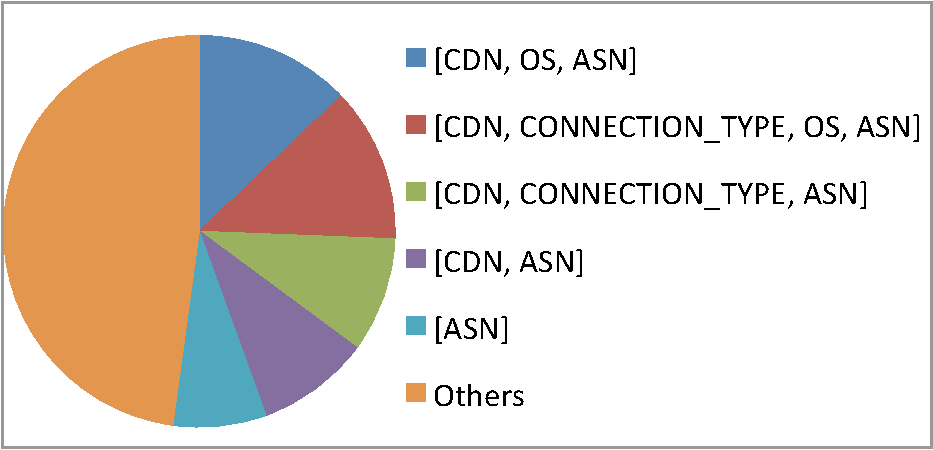
\includegraphics[width=0.4\textwidth]{figures/optimal_AC_distribution.pdf}
}
\subfigure[Prevalence of pair of (session under prediction, optimal AC).]
{
        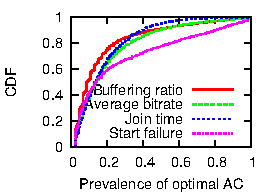
\includegraphics[width=0.33\textwidth]{figures/optimal-prevalence.pdf}
}
\subfigure[Persistence of pair of (session under prediction, optimal AC).]
{
        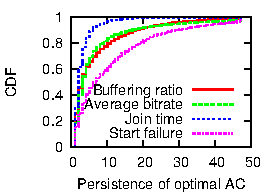
\includegraphics[width=0.33\textwidth]{figures/optimal-persistence.pdf}
}
\tightcaption{Dynamics of the optimal AC. (a) gives coverage of optimal ACs (for each AC, the fraction of sessions of which this AC is the optimal AC).
(b) gives prevalence of pair of (session under prediction, optimal AC) (the fraction of time that the finest group has this optimal AC).
(c) gives persistence of pair of (session under prediction, optimal AC) (i.e., the longest continuous duration where a finest group has the same optimal AC).}
\label{fig:optimal-ac-dynamics}
\end{figure}

\myparatight{Optimal AC} We find that the optimal AC (the aggregation that gives minimal prediction error) is in many cases neither the finest nor the coarsest one, and, in addition, is highly dynamic:
 
\begin{packeditemize}
	\item {\it No single optimal AC:} Figure~\ref{fig:optimal-ac-dynamics}-(a) shows the coverage of optimal ACs, i.e., the fraction of time for which a given AC is the optimal AC. Note that there is no single optimal AC. For example, the finest group only has coverage about 20\% and no coarsest grain AC (single attribute) is among the top 5. This implies that the optimal AC is often in between.
	\item {\it No temporally prevalent optimal AC:} Figure~\ref{fig:optimal-ac-dynamics}-(b) shows the prevalence of the $($\emph{session-under-prediction, optimal AC}$)$ pairs, i.e., the fraction of time the fines group of sessions has the same optimal AC. Note that $70\%$ pairs only last for less than $20\%$ of time. This implies that there is no single or a small set of optimal ACs that can cover most sessions.
	\item {\it Highly dynamic optimal ACs:} Figure~\ref{fig:optimal-ac-dynamics}-(c) shows the persistence of the $($\emph{session-under-prediction, optimal AC}$)$ pairs, i.e., the longest continuous duration where the finest group has the same optimal AC. Only 40\% of pairs last for more than 10 minutes. This suggests that even with a reactive strategy will be challenging to track the optimal ACs.
\end{packeditemize}


